\documentclass{article}
\usepackage[parfill]{parskip}
\usepackage{graphicx}
\usepackage[T1]{fontenc}
\usepackage{gentium}
\usepackage{amsfonts} 
\usepackage{listings}

\lstset{basicstyle=\ttfamily, keywordstyle=\bfseries, columns=fullflexible}

\author{Stian Onarheim}
\title{RFMA310-1 20H Diskret matematikk Hjemmeeksamen}

\begin{document}
\maketitle
\newpage
\tableofcontents
\newpage

\section{Abstract}
My submission for the homeexam in the subject RFMA310-1 20H Diskret matematikk.

\section{The Elgamal Encryption Algorithm}
The Elgamal Encryption Algorithm build upon the concept of \textit{The Discrete Logarithm Problem}. With a cyclic group $G$, and a unique $k \in \mathbb{Z}$, there exists a generator $g$ so that every element $a \in G$ can be written as $a = g^k$. The challenge is to find the number $k$ in $a = g^k$ when $a, G$ and $g$ is given. The difficulity in solving the logarithm is dependent on a good choice of a cyclic group and a corresponding generator.

The person who wants to receive an ecrypted text, starts by creating a private and public key. The public key consists of four elements. A cyclic group $G := (\mathbb{Z}/p)^x$ under multiplication, where $p \in Spec(\mathbb{Z})$, the group's order $q$, a generator from the group $G$, and an element $h := g^x \in G$, where $x \in G$ is the private key. The elements ($G, q, g, h$) makes the pulbic key, and is shared with the sender.

The sender will use the public key to encrypt a message $m \in G$. The sender also creates their own private key $y \in G$. The sender computes the shared secret $s := h^y \in G$. The cipertext consists of two elememts $c_1, c_2 \in G$, which are commputed as $c_1 := g^y, c_2 := m \cdot s$. The ciphertext ($c_1,c_2$) is sent to the receiver.

The receiver has now received the ciphertext ($c_1, c_2$) from the sender, and has every tool it needs to decrypt the message. It starts by computing the shared secret $s$ which was used by the sender under encryption. The sender computed it as $s := h^y \Leftrightarrow s:= g^{xy}$. Since the ciphertext element $c_1 = g^y$, the shared secret $s$ can be computed as $s := c_1^x \Leftrightarrow g^{yx}$. The plaintext $m$ is computed as $m := c_2 \cdot s^{-1}$, so the shared secret's inverse needs to be computed. Using Lagrange's theorem, the inverse can be computed as $s^{-1} := c_1^{q-x}$.

As the cyclic group $G$ has a multiplication operator, its unit element $e := 1$. The plaintext is computed as $c_2 \cdot s^{-1} \Leftrightarrow (m \cdot s) \cdot s^{-1} \Leftrightarrow m \cdot e \Leftrightarrow m$. Both parties are now left with the same plaintext message.

\newpage
\section{The source code}
I have implemented Elgamal in python as it supports enormous numbers within its default libraries. Before encrypting the plaintext, I convert its characters to ASCII values and concatenates them together.\\

The message to be encrypted has to be an element of the cyclic group $G$, creating a limit to the message's length. To support longer messages, the message is divided into blocks smaller than $G$'s order. As the ASCII values varies from one to three digits, zeroes are appended at the beginning to make every value the same length. This is needed to make decryption easier. In Figure \ref{blocks}, the blue block represents an example of this padding. 

Each block is encrypted seperately with the Elgamal protocol. The ciphertexts consists of two elements ($c_1, c_2$), which combined are two times longer than the message itself. After decryption, we are left with the same blocks as before the encryption. The blocks' length are strategically a multiple of 3, which makes it easier to deconstruct them back into characters.  

The Elgamal encryption algorithm faces a problem with larger numbers. It performs the computation of $a^b\ (mod\ n)$ several places, where $a^b$ can become an enormous number and requires more computation time. To handle this problem and achieve fast computation times, the course book \textit{Discrete Mathematics and its Applications} includes pseudocode for a \textit{Fast Modular Exponentiation} function.

As it is hard to define a good cyclic group and a generator, they are static in my implementation. The sender and receiver's private keys are randomly generated for each block.
\begin{figure}
    \centering
    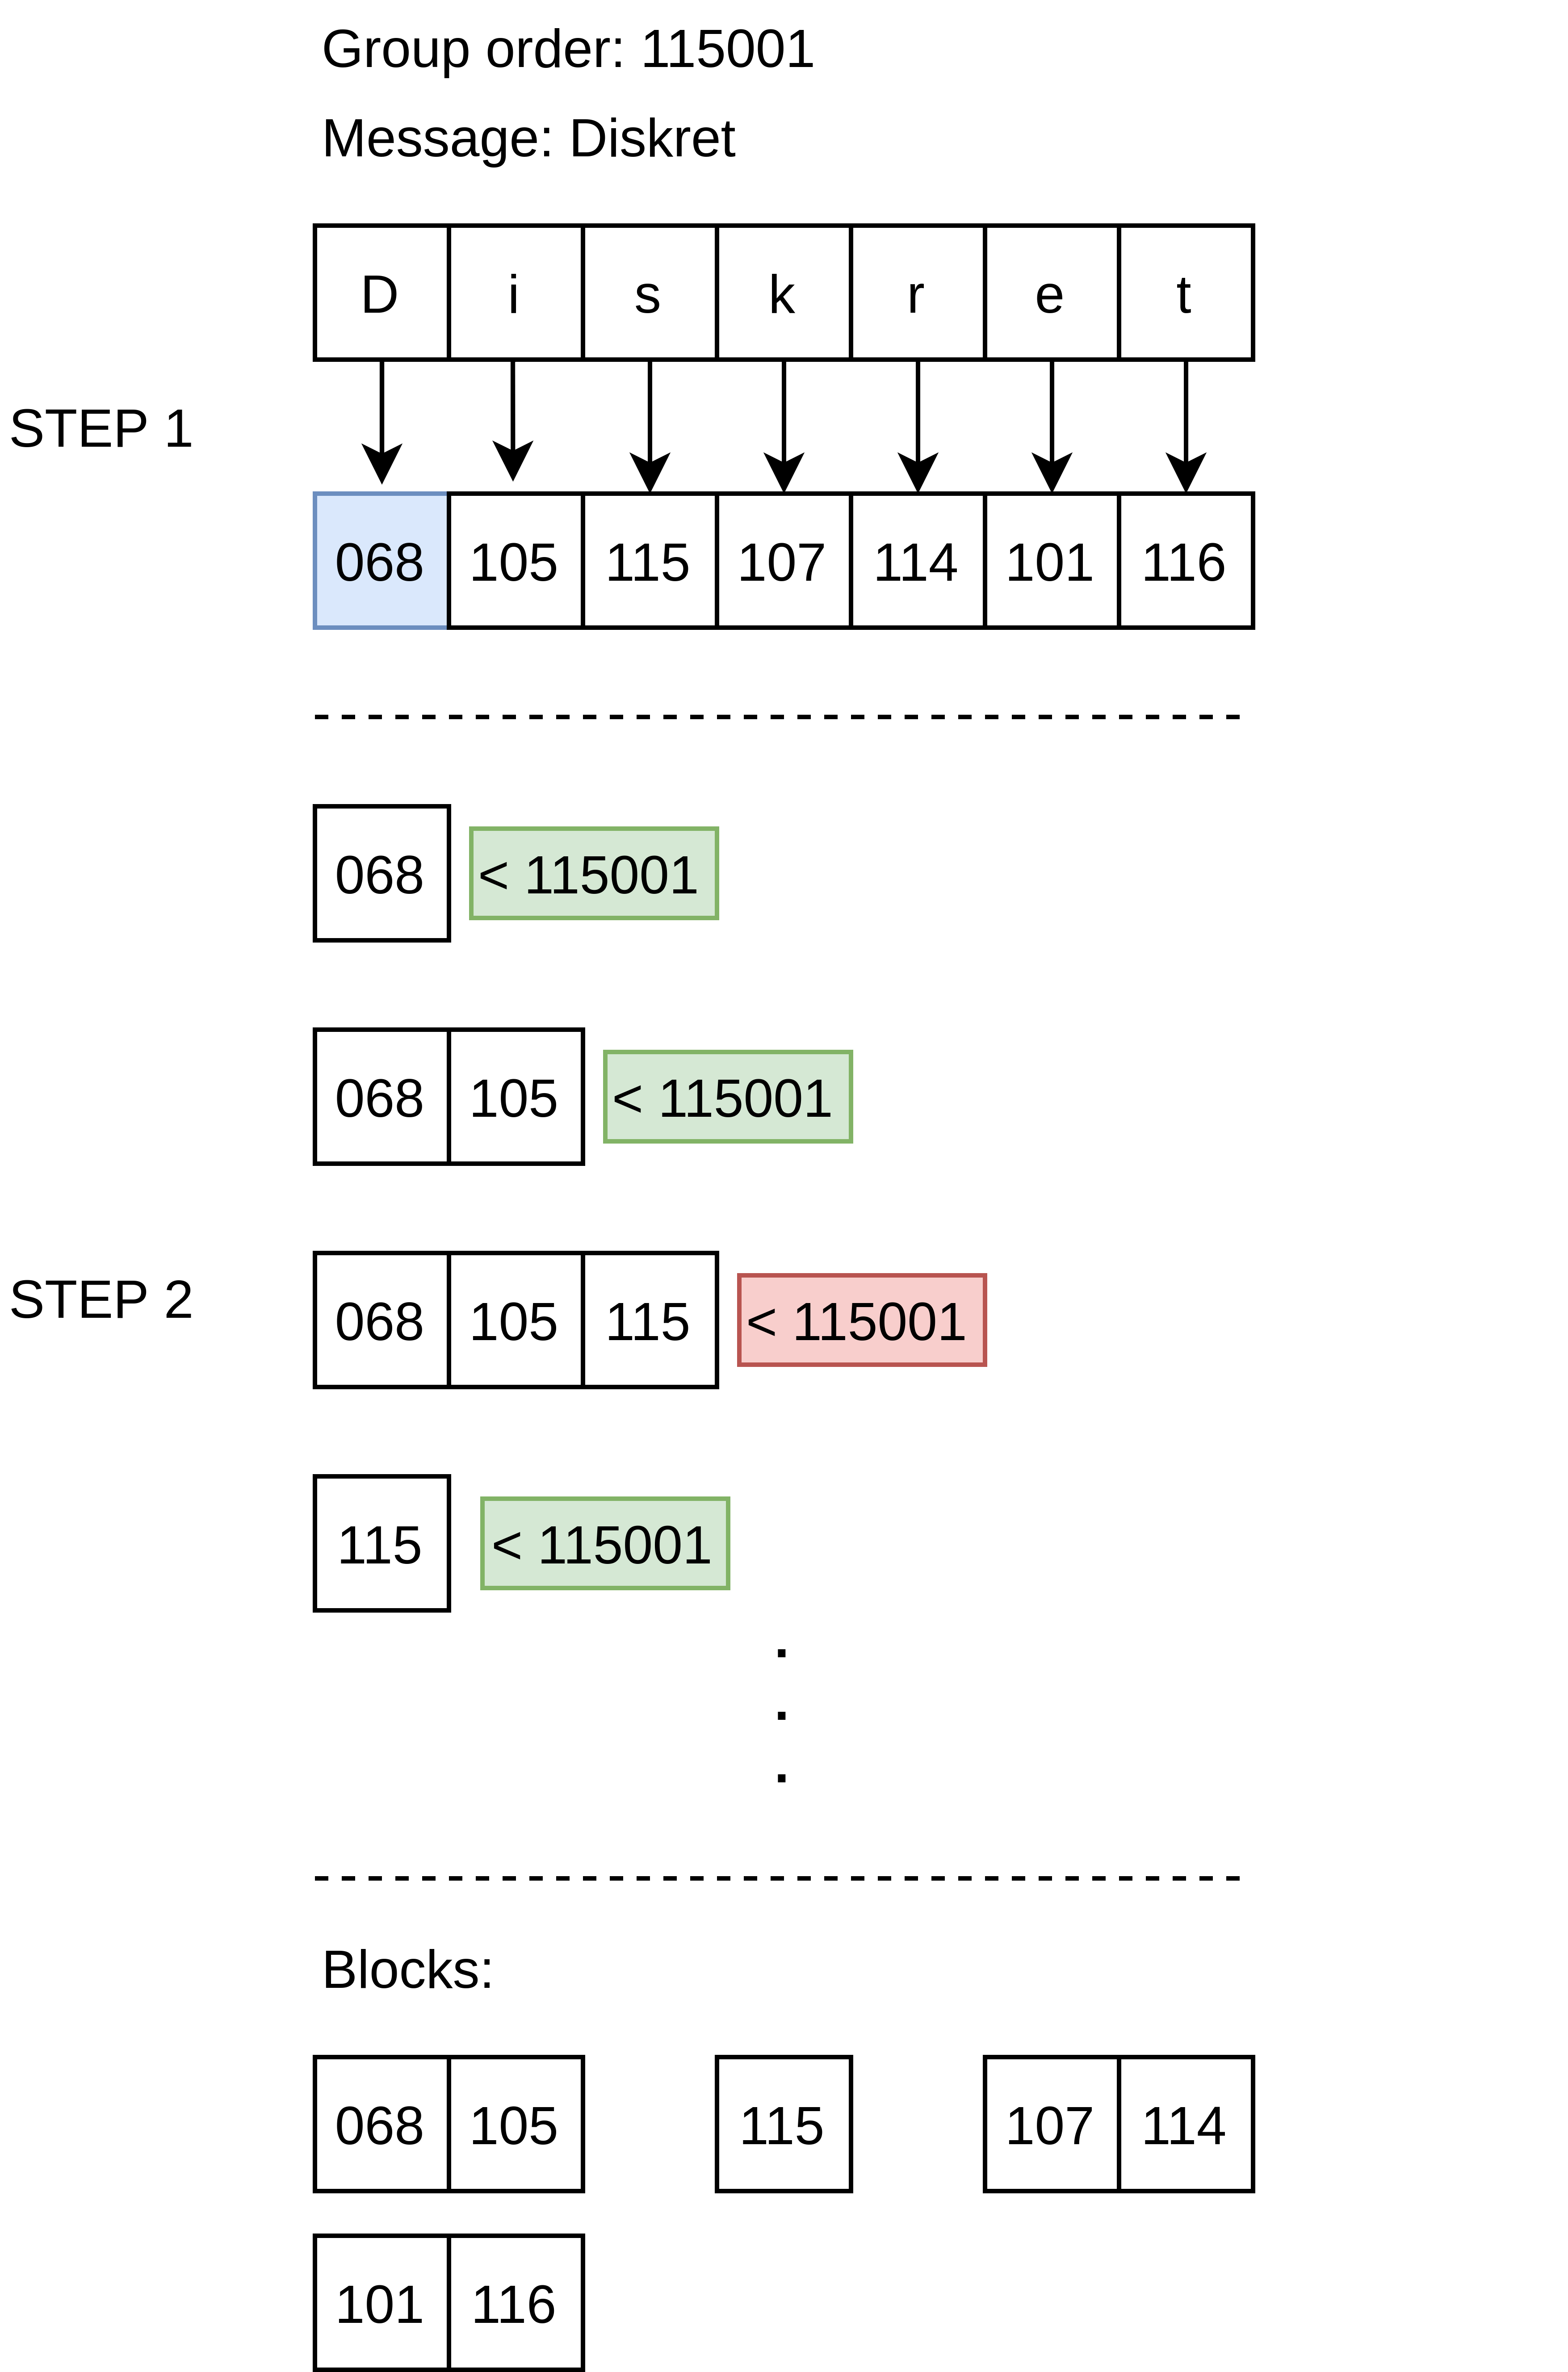
\includegraphics[scale=0.1]{img/construct-blocks.png}
    \caption{Example of constructing blocks out of the message.}
    \label{blocks}
\end{figure}

\newpage
\section{Elgamal Implementation Python Source Code}
\begin{lstlisting}[language=Python,breaklines=true,showspaces=false]
import random
import sys, getopt

###############################
## fastModularExponentiation ##
###############################

def fastModularExponentiation(generator, exponent, mod):
    x = 1
    power = generator % mod
    binaryString = bin(exponent)

    for i in binaryString[::-1]:
        if i == '1':
            x = (x * power) % mod
        power = (power * power) % mod
    return x


################
## addPadding ##
################

def addPadding(a):
    if len(a) % 3 != 0:
        if len(a) % 3 == 1:
            return "00" + a
        else:
            return "0" + a
    else:
        return a

#####################
## constructBlocks ##
#####################


def constructBlocks(message, prime):
    if prime < 131:
        sys.exit("Your Primenumber is less than the minimum (131).")

    retList = []
    i = 0
    while i < len(message):
        tempValue = addPadding(str(ord(message[i])))
        for j, k in enumerate(message[(i+1):len(message)], 1):
            nextChar = addPadding(str(ord(k)))
            concatenateValue = tempValue + nextChar

            if int(concatenateValue) > prime:
                break
            else:
                tempValue = concatenateValue
                i += 1

        retList.append(tempValue)
        i += 1
    return retList;

#######################
## deconstructBlocks ##
#######################

def deconstructBlocks(blocks):
    retString = ""
    for i in blocks:
        for j in range(int(len(str(i))/3)):
            retString += chr(int(str(i)[j*3:3*(j+1)]))

    return retString

#############
## encrypt ##
#############

def encrypt(prime, message, privateKey):
    q = prime - 1
    generator = 150 

    x = privateKey
    h = fastModularExponentiation(generator, privateKey, prime)

    y = random.randint(1, q)

    s = fastModularExponentiation(h, y, prime)

    c1 = fastModularExponentiation(generator, y, prime)

    c2 = fastModularExponentiation((int(message) * s), 1, prime)

    retList = [c1, c2]

    return retList

################
## decryption ##
################

def decryption(prime, privateKey, encryptedList):
    q = prime - 1
    c1 = encryptedList[0]
    c2 = encryptedList[1]
    x = privateKey

    inverse = fastModularExponentiation(c1, (q - x), prime)
    decryptedMessage = fastModularExponentiation((c2 * inverse), 1, prime)

    return addPadding(str(decryptedMessage))

def main():
    inputFile = ""
    outputFIle = ""
    printing = True

    #with open('main.cpp', 'r') as file:
            #stringMessage = file.read()

    stringMessage = "Diskret?"

    prime = 58021664585639791181184025950440248398226136069516938232493687505822471836536824298822733710342250697739996825938232641940670857624514103125986134050997697160127301547995788468137887651823707102007839
    blocks = constructBlocks(stringMessage, prime)

    encryptedList = []
    privateKeys = []
    for i in blocks:
        currentPrivateKey = random.randint(1, (prime - 1))
        privateKeys.append(currentPrivateKey)
        encryptedList.append(encrypt(prime, i, currentPrivateKey))

    decryptedList = []
    for i, j in enumerate(encryptedList, 0):
        decrypted = decryption(prime, privateKeys[i], j)
        decryptedList.append(decrypted)

    decryptedMessage = deconstructBlocks(decryptedList)

    if stringMessage == decryptedMessage:
        print("Success!")
    else:
        print("Failed.")

    if printing:
        print("Plaintext:", stringMessage)
        print("Prime Number:", prime, "\n")
        print("Blocks: (", len(blocks), ")")
        for i in blocks:
            print(i, end = " ")
        print("\n")

        print("Encrypted Blocks:")
        for i in encryptedList:
            print(i, end = " ")
        print("\n")

        print("Decrypted Blocks:")
        for i in decryptedList:
            print(i, end = " ")
        print("\n")

        print("Decrypted Message: \n" + decryptedMessage)

if __name__ == '__main__':
    main()

\end{lstlisting}

\newpage
\nocite{*}
\bibliography{main}{}
\bibliographystyle{plain}

\end{document}
